
\chapter{Search Strategy}
\label{ch:SearchStrategy}
%Deep thoughts go here.
This chapter will describe the major backgrounds and outline a search strategy used in the analysis.  The kinematic regions for the signal will be defined as well as the introduction of neural networks to assist with the separation of signal and background like events.


\section{Major Backgrounds}
There are a large number of Standard Model processes that can end up in the signal region and share a similar final state topology as the studied signal process, $t\bar{t}\rightarrow b l \nu q \gamma$.  All of these processes are modeled with Monte Carlo( MC) simulation, with the exception of particles that fake other particles (leptons and photons) which are done using data-driven techniques because they are poorly modeled with MC.  A full list of the Monte Carlo samples used for each background can be found in Appendix \ref{app:MC_Samples}. 

The dominant backgrounds in this search are Standard Model $t\bar{t}$, Standard Model $t\bar{t}+\gamma$, as well as W+jets and W+jets with an associated photon (W+jets+$\gamma$).  These along with minor backgrounds (Standard Model single top events, Z+jets (Z+jets+$\gamma$), $t\bar{t}$+Vector Boson, diboson) are all modeled with MC and some data-driven estimates and corrections are applied.  The various backgrounds modeled in this search as summarized here:

\begin{description}
\item[\textbf{SM Processes}:]  SM $t\bar{t}$, W+jets, Z+jets, single top, diboson, $t\bar{t}$+V are modeled with MC simulations.  Control and validation regions are designed to test preformance of the largest of these background proceses, $t\bar{t}$ and W+jets.  A discussion of the modeling of the major SM processes without photons and a derivation of additional scale factors for these processes is shown in Section \ref{sec:BKGnoPho}.

\item[\textbf{SM Processes with an associated photon}:] SM + associated photon processes: $t\bar{t}+\gamma$, W+jets+$\gamma$, Z+jets+$\gamma$ are modeled with MC simulation and overlap removal is applied to the SM processes to remove events with similar phase spaces since these processes are a subset of the SM process.  MC simulations are created with additional statistics for these processes.  Additional details are presented in Section \ref{sec:BKGPho}.

\item[\textbf{Fake Leptons}:] Non-prompt or fake electrons and muons can arise from semi-leptonic decay of $b$ and $c$ quarks.  For electrons additional contributions from photon conversions and jets in the electromagnetic calorimeter can lead to lepton fakes.  Muons can be faked via energetic showers in the hadronic calorimeter or from hadrons that punch-through the hadronic calorimeter.  The matrix method is used to estimate the number of events with fake leptons as described in Section \ref{sec:FakeLep}.

\item[\textbf{Fake Photons}:] The number of events with fake photons are estimated using a $Z\rightarrow e^+ e^-$ tag-and-probe method discussed in Section \ref{sec:FakePho}.  Further, the ABCD method is used in Section \ref{sec:FakePho2} to estimate the number of fake photon events that arise from a jet faking a photon.

\end{description}
\subsection{Overlap Removal}
\label{sec:OverlapRemoval}
Tracks and energy deposits within the detector can, in some cases, be used to reconstruct multiple objects.  To prevent using these tracks and deposits multiple times a standard overlap removal procedure is applied to objects.  First, electrons that share tracks with any other electrons are removed.  Any electron sharing a track with a muon is then also removed.  Any jet that is found within  $\Delta R < 0.2$ of an electron is removed.  Then any jet with less than 3 tracks associated with it within $\Delta R < 0.2$ of a muon object is removed.  After that any muon found withing $\Delta R < 0.4$ of a jet is removed and any photon within $\Delta R < 0.4$ of an electron or muon object is removed. % Any jet found within $\Delta R < 0.4$ of a \textit{Loose} photon is also removed. 

\subsection{Duplicate Event Removal}
As specialized higher statistic samples are used for processes with prompt photons a double counting of events could occur with the nominal MC samples.  For example, in addition to the $t\bar{t}$ sample a sample of $t\bar{t}+\gamma$ events are used.  This is true for the W+jets/Z+jets and special samples of W+jets+$\gamma$ and Z+jets+$\gamma$.  Therefore a truth based matching scheme is used to remove events in the nominal samples that match with the photon types produced in the specialized $+\gamma$ samples i.e., they contain a truth photon that does not originate from a hadron or lepton.

\section{Event Selection}
This analysis is searching for $t\bar{t}$ candidate events where one of the top quarks decays through the most common decay path (a W boson that decays leptonically to an electron or muon and a bottom quark) and the other through the FCNC diagram to an up type light quark and a photon.  The selected decay path is then $t\bar{t} \rightarrow Wbq\gamma \rightarrow l\nu b q \gamma$ such that the final state will contain at least two jets exactly one of which is b-tagged using the MV2c10 algorithm, exactly one massive lepton (an electron or muon), exactly one highly energetic photon, missing transverse energy from the neutrino, and a large transverse W mass.  The transverse W mass requirement selects events that have a lepton and $\slashed{E}_T$ which are consistent with a leptonically decaying W boson, defined as:
\[ m_T^{W} =  \sqrt{2\times p_{T_l}\times \slashed{E}_T \times (1 - \text{cos}(\phi_l -\phi_{\text{MET}}))}\]
which is largest when the lepton and missing transverse energy are close in $\phi$ as would be expected from the decay products of a boosted W boson.  Events are selected loosely to include all possible kinematic regions of interest and then skimmed down to the individual regions for various studies.  This includes events that will not enter the signal region such as events with 0 photons or events with 0 b jets that are used to derive and test scale factors on the largest background samples and account for mismodeling of MC simulations. 

For the events that have a chance of entering the final Signal Region i.e., events with exactly one b-tagged jet and exactly one photon, a neural network analysis is preformed to help separate the signal from the background using a variety of high dimensional cuts.  The neural network training and testing are described in Section \ref{sec:NN}.  The neural network is then applied to all events with 1 b-tagged jet and 1 photon and greatly increases signal purity while separating out the most dominant backgrounds, in particular $t\bar{t}$ and $t\bar{t}+\gamma$.


%Something about neural network to feed into that section



%%%%%%%%%%%%%%%%%%%%%%%%%%%%%%%%%%%%%%%%%%%%%%
%%%%%%%%%  									        	 %%%%%%%%
%%%%%%%%%                     Start of Neural Net Section                                           %%%%%%%%
%%%%%%%%%										 %%%%%%%%
%%%%%%%%%%%%%%%%%%%%%%%%%%%%%%%%%%%%%%%%%%%%%%

\section{Event Classification: Neural Network Optimization}
\label{sec:NN} 
To help distinguish signal events from the majority of background events neural networks were employeed for event classification.  Neural networks are multivariate methods that take a variety of inputs and output a number between 0 and 1.  The output value is a discriminating variable that will be used to classify events and determine which events make it into the final Signal Region selection.  Signal-like events accumulate towards 1 while background-like events cluster around 0.  Two neural networks are trained, one for the electron+jets final state and one for the muon+jets final state.  This section will discuss the neural network studies completed and their uses in the search for FCNC events.  

\subsection{Input Variables}
A wide variety of input variables to the neural network were studied in detail.  Studies were done using only low level variables such as the kinematic variables  ($p_T$, $\eta$, $\phi$, $E$)  of the physics objects in the signal region.  This was done as a complex enough neural network should be able to figure out useful high level/event level variables (i.e. invariant masses, geometric separations) but in practice a combination of some of these low level variables and high level variables used as inputs to the neural network proved to give the best separation and projected limits.  Using physical intuition to guide the neural network proved to be a valuable tool.

Combinations of 29 input variables were tested to start with however variables such as $\eta$ and $\phi$ tend to not have significant weights in the neural network and are left out in favor the the high level variables that include them (e.g., $\Delta R$ values).  A measure of how different the variables are between signal and background is the Separation.  Table \ref{tab:Separations} shows the separation values for the variables that are inputs to the final neural network.  Comparisons between the shapes of the input variables for the $\mu$+jets channel are shown in Figures \ref{fig:VarPlots1}, \ref{fig:VarPlots2}, and \ref{fig:VarPlots3}

\begin{table}[]
\begin{center}
{\renewcommand{\arraystretch}{1.2}
\begin{tabular}{ccc}
\hline
Variable  &  Separation e+jets   & Separation $\mu$+jets   \\  \hline 
$p_T (\gamma)$            &  22.97   & 24.01	\\
$m_{q\gamma}$           &   22.65 &  28.31	\\
$\gamma_{\text{iso}}$   &  18.62   &  41.32	\\   
$m_{bW} $                    &  11.10   &  11.70 	\\
$m_{l\gamma}$             &  9.00  &   7.51	\\
$\Delta R_{j\gamma}$ &  4.59   &  5.66	\\
$\Delta R_{b l}$            &  4.99   &  4.47 	\\
$m_{T}^{W}$              &   3.16  &   3.37	\\
$S_T$                            &  3.78   &  3.32 	\\
$n_{\text{jets}}$         &  1.70   &   2.03	\\
$\chi^{2}_{W}$           &  1.37 &   1.91	 	\\
$p_T (q)$                      &  2.46    &  2.82	\\
$\Delta R_{l \gamma}$ &   1.40 &  1.19		\\
E (lepton)                       &  0.86  &  0.89	\\	
$\slashed{E}_T  $          &   0.47  & 0.70 	\\
$p_T (b)$                       &  0.51    &  0.53	\\ \hline
\end{tabular}
\caption{Separation of normalized variables between signal and bacground in the e+jets and $\mu$+jets channels for the variables used as input to the final neural network.  }
\label{tab:Separations}
}
\end{center}
\end{table}

\[ \text{Separation} = \sum_{i}^{bins} \frac {n_{s i}-n_{b i}}{n_{s i}+n_{b i}}\]

Typically the kinematic variables with photon information have the biggest separation values.  This is expected because the signal photon comes directly from the decay of a top quark and is much more energetic than background photons.  Shape comparison plots for the $e$+jets channel and additional plots for other investigated variables are shown in Appendix \ref{app:NN}.  The largest difference in separation between the $e$+jets and $\mu$+jets channels is the photon isolation value.  This is due to the fact that all backgrounds are included and fake photon contamination from a large Z+jets background are expected.  Both networks preform similarly in their separation of signal and background events.  The network is able to learn and compensate for this behavior with the help of other variables that include the lepton and photon: $\Delta R_{l \gamma}$ and $m_{l\gamma}$.

The neural networks are trained on MC events that have a chance of being in the signal region after basic event level cuts and optimized for signal significance.  Only events with 1 photon ($>15$ GeV) and 1 bjet (MV2c10 77\% working point) are classified by the neural network.  The 77\% working point was chosen by training the neural network on events with only 1 bjet at each working point: 70\%, 77\%, and 85\% and picking the network and working point with the best estimated significance.  The b-tagging neural network study is shown in Section \ref{sec:btagNN}

\begin{figure}[h!]
\centering
\subfloat[$\gamma_{iso}$ topo$E_{T}$cone40]{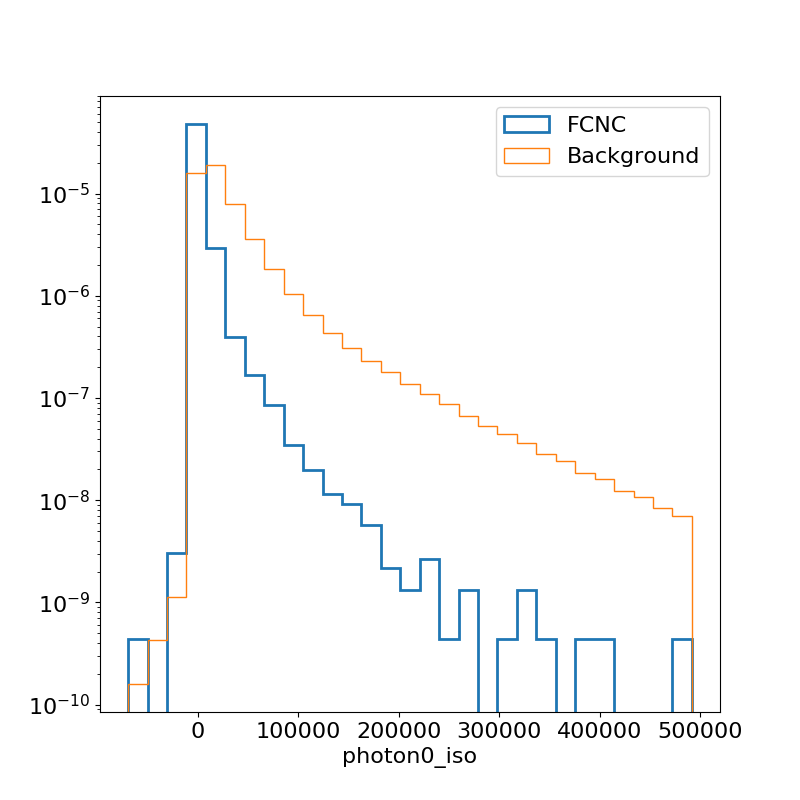
\includegraphics[width=.4\columnwidth]{../ThesisImages/SearchStrategy/varplots/photon0_iso.png}}\hfil
\subfloat[$\gamma_{p_T}$]{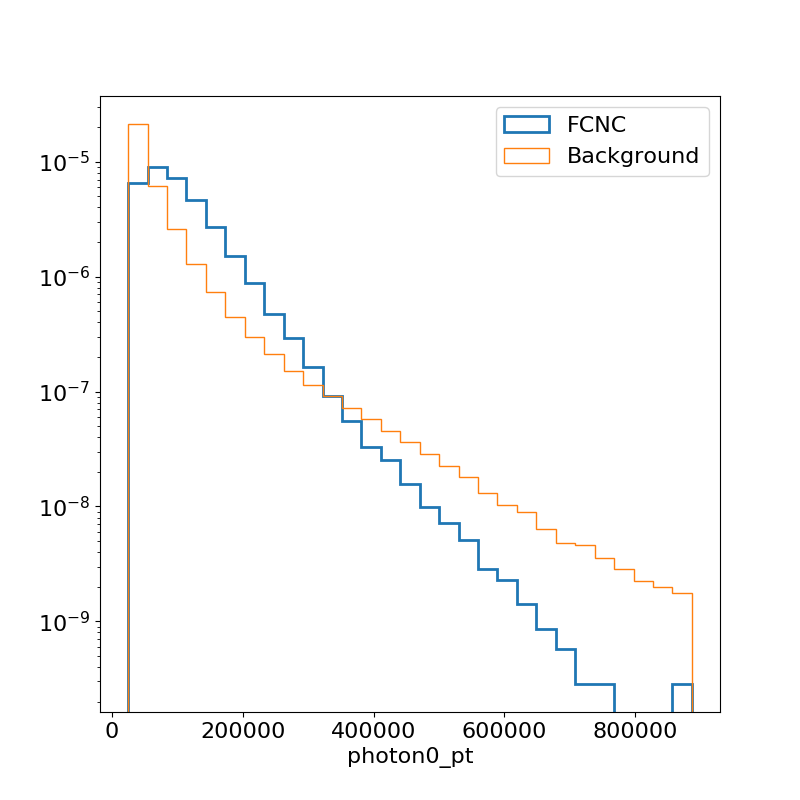
\includegraphics[width=.4\columnwidth]{../ThesisImages/SearchStrategy/varplots/photon0_pt.png}}
\vspace{-4.5mm}
\subfloat[$m_{q \gamma}$]{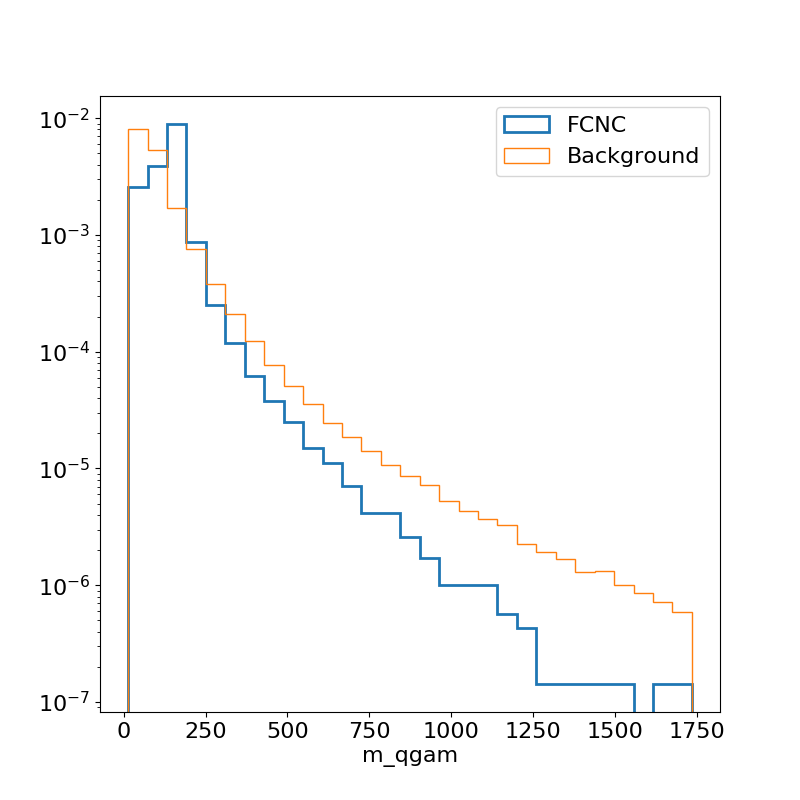
\includegraphics[width=.4\columnwidth]{../ThesisImages/SearchStrategy/varplots/m_qgam.png}}\hfil
\subfloat[$m_{l \gamma}$]{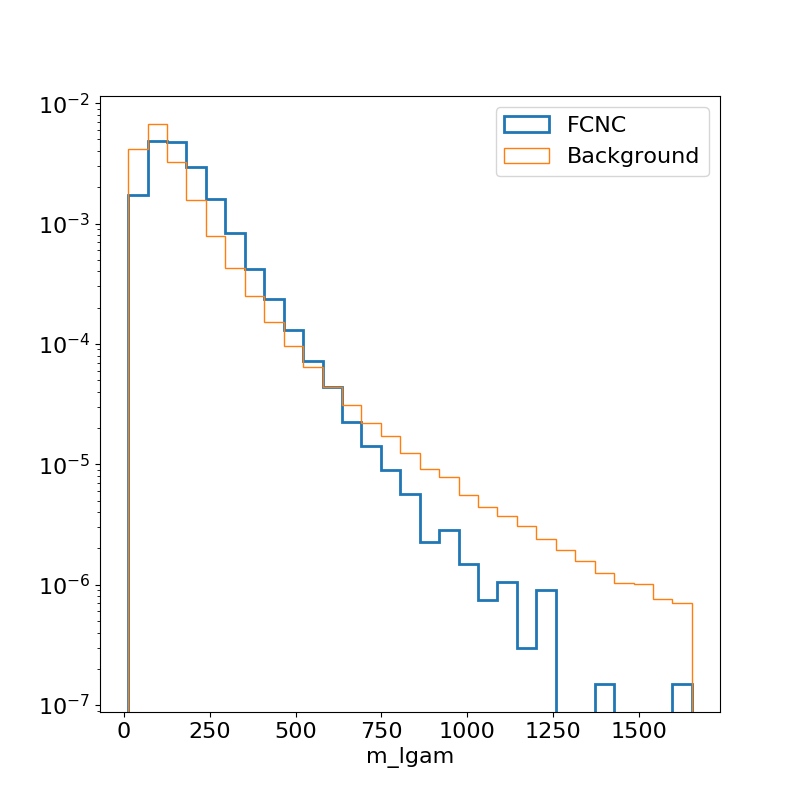
\includegraphics[width=.4\columnwidth]{../ThesisImages/SearchStrategy/varplots/m_lgam.png}}   
\vspace{-4.5mm}
\subfloat[$m_{bW}$]{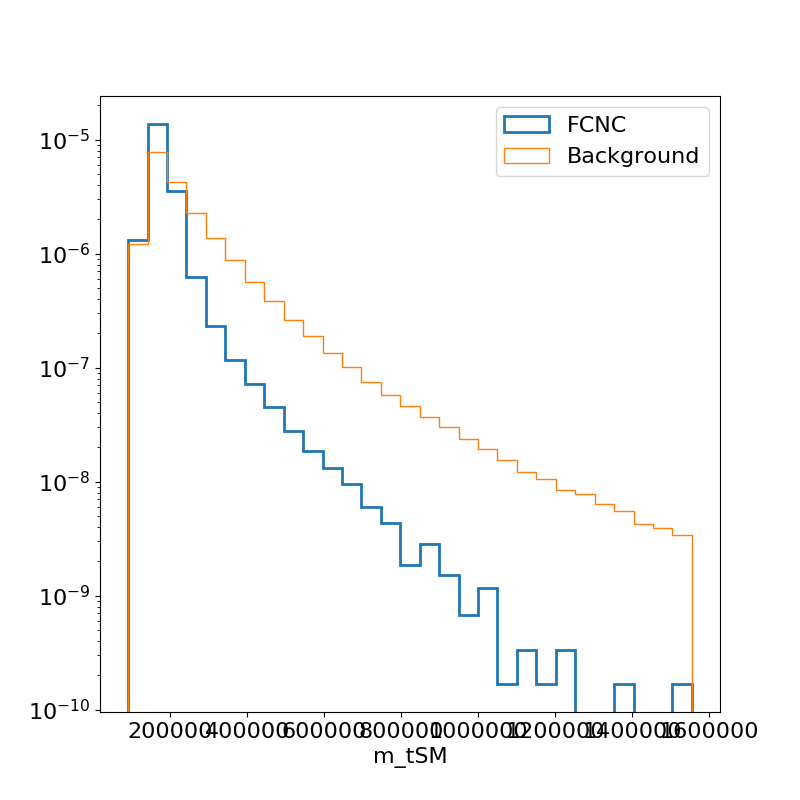
\includegraphics[width=.4\columnwidth]{../ThesisImages/SearchStrategy/varplots/m_tSM.png}}\hfil
\subfloat[$\Delta R_{j\gamma}$]{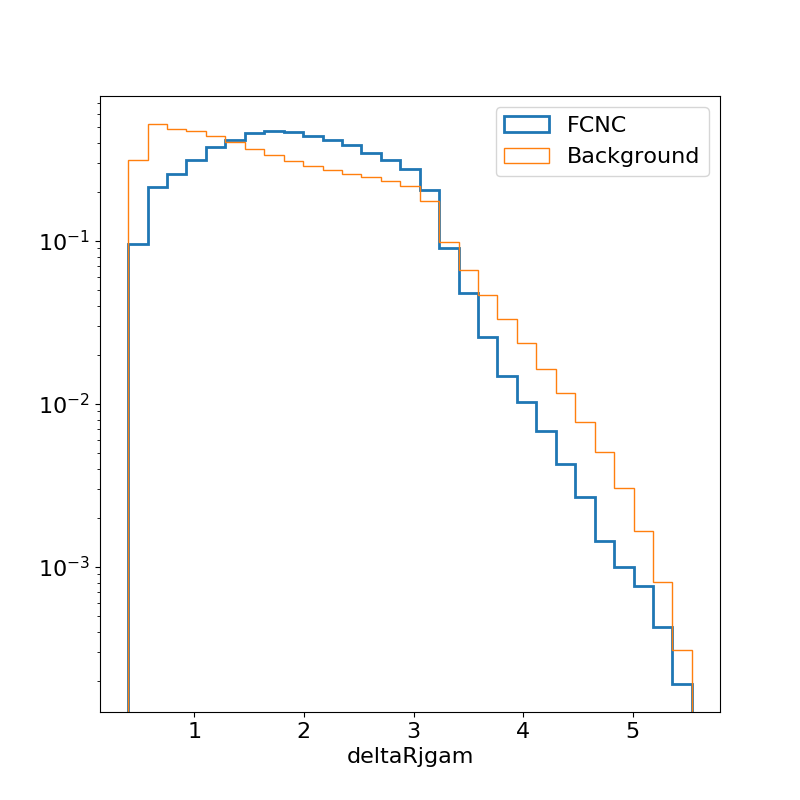
\includegraphics[width=.4\columnwidth]{../ThesisImages/SearchStrategy/varplots/deltaRjgam.png}}
\caption{Normalized variables showing the shapes of neural network input variables for the $\mu$+jets channel: $\gamma_{iso}$ topo$E_{T}$cone40, $\gamma_{p_T}$, $m_{q \gamma}$, $m_{l \gamma}$, $m_{bW}$, and $\Delta R_{j\gamma}$ }
\label{fig:VarPlots1}
\end{figure}



\begin{figure}[h!]
\centering
\subfloat[$\Delta R_{b l}$]{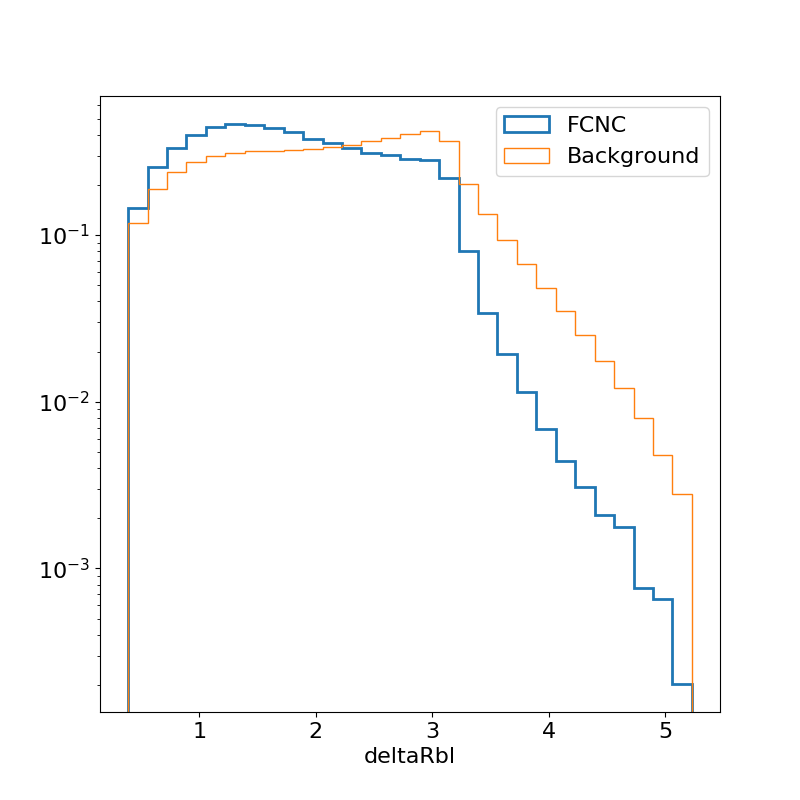
\includegraphics[width=.4\columnwidth]{../ThesisImages/SearchStrategy/varplots/deltaRbl.png}}\hfil
\subfloat[$m_{T}^{W}$ ]{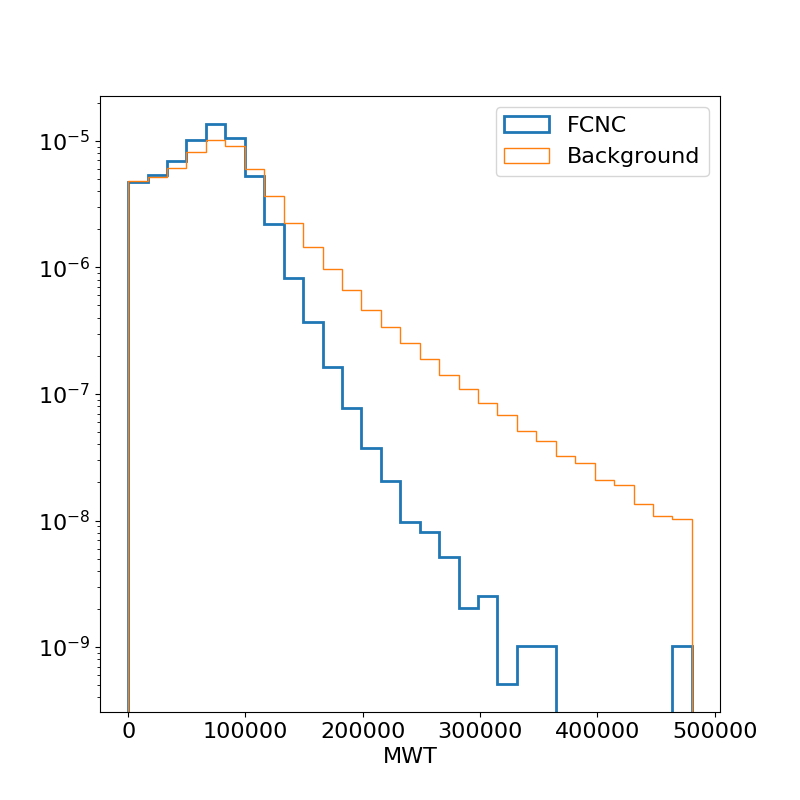
\includegraphics[width=.4\columnwidth]{../ThesisImages/SearchStrategy/varplots/MWT.png}}
\vspace{-4.5mm}
\subfloat[$S_T$]{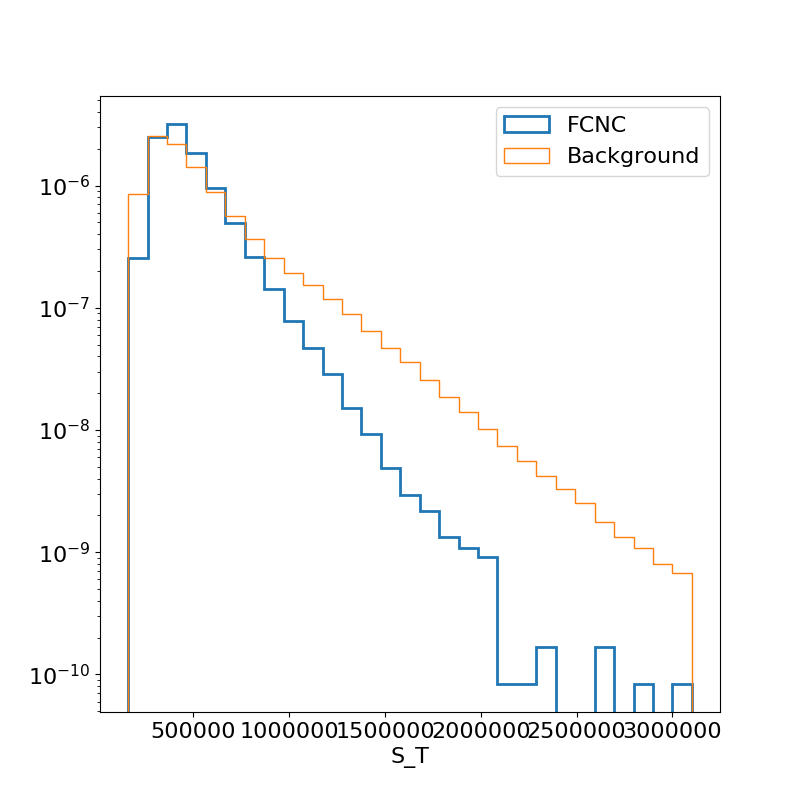
\includegraphics[width=.4\columnwidth]{../ThesisImages/SearchStrategy/varplots/S_T.png}}\hfil
\subfloat[$n_{\text{jets}}$]{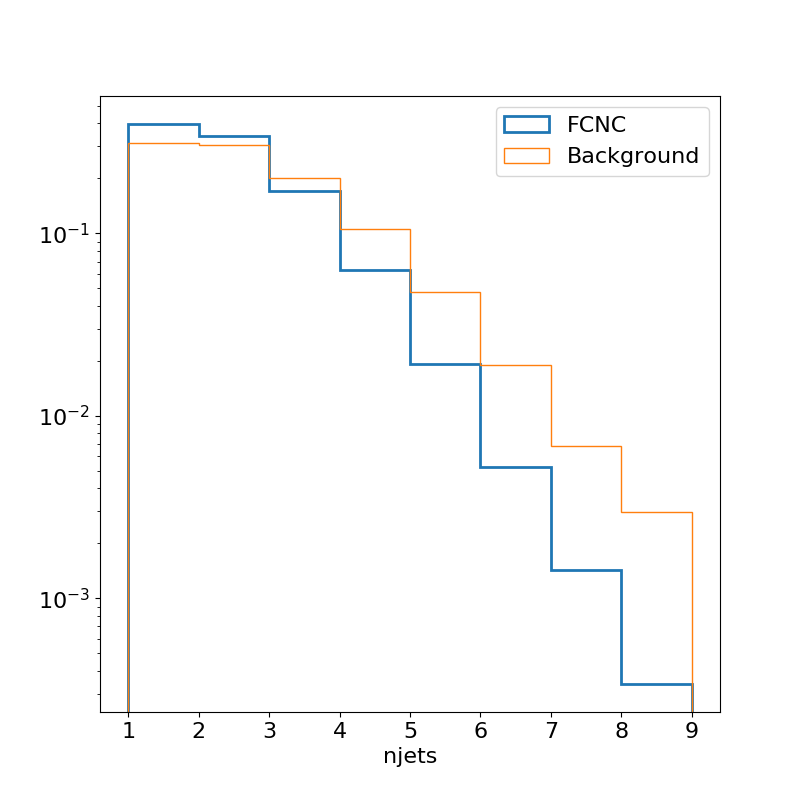
\includegraphics[width=.4\columnwidth]{../ThesisImages/SearchStrategy/varplots/njets.png}}   
\vspace{-4.5mm}
\subfloat[$\chi^{2}_{W}$]{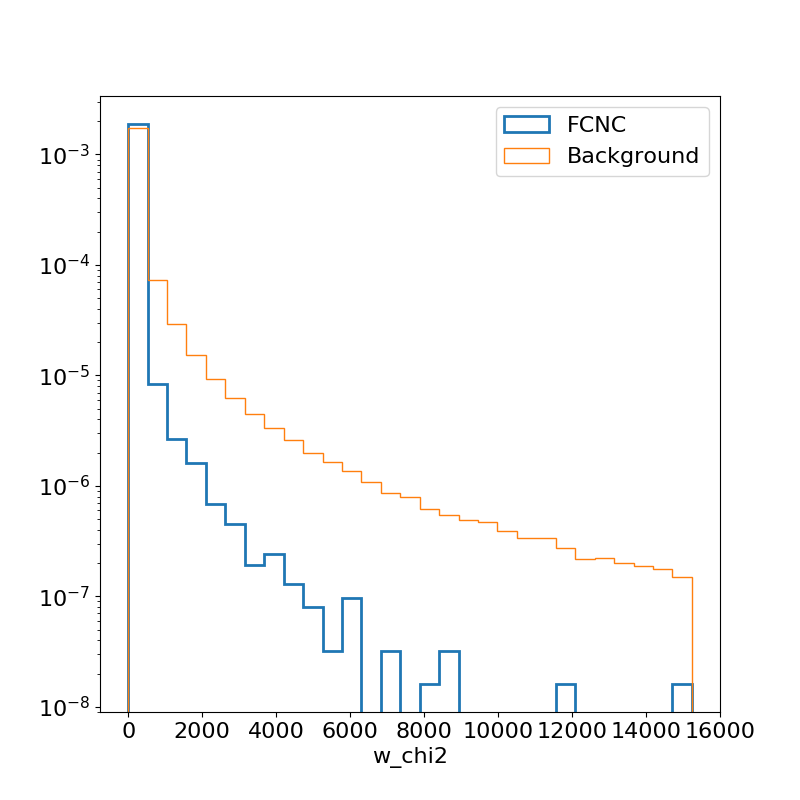
\includegraphics[width=.4\columnwidth]{../ThesisImages/SearchStrategy/varplots/w_chi2.png}}\hfil
\subfloat[$p_T (q)$]{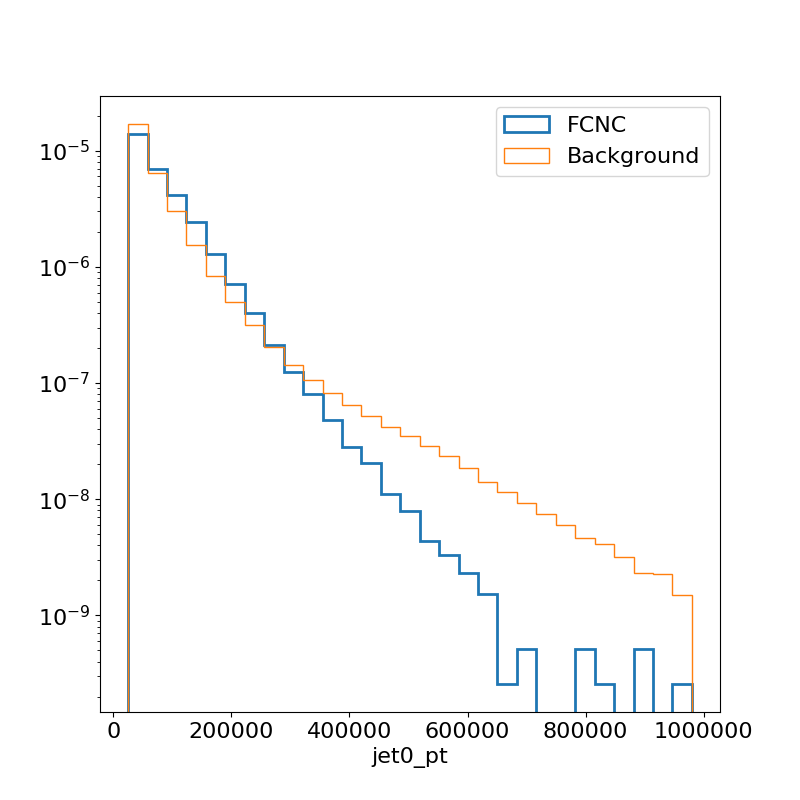
\includegraphics[width=.4\columnwidth]{../ThesisImages/SearchStrategy/varplots/jet0_pt.png}}
\caption{Normalized variables showing the shapes of neural network input variables for the $\mu$+jets channel: $\Delta R_{b l}$, $m_{T}^{W}$ , $S_T$, $n_{\text{jets}}$, $\chi^{2}_{W}$, and $p_T (q)$}
\label{fig:VarPlots2}
\end{figure}

\begin{figure}[h!]
\centering
\subfloat[$\Delta R_{l \gamma}$]{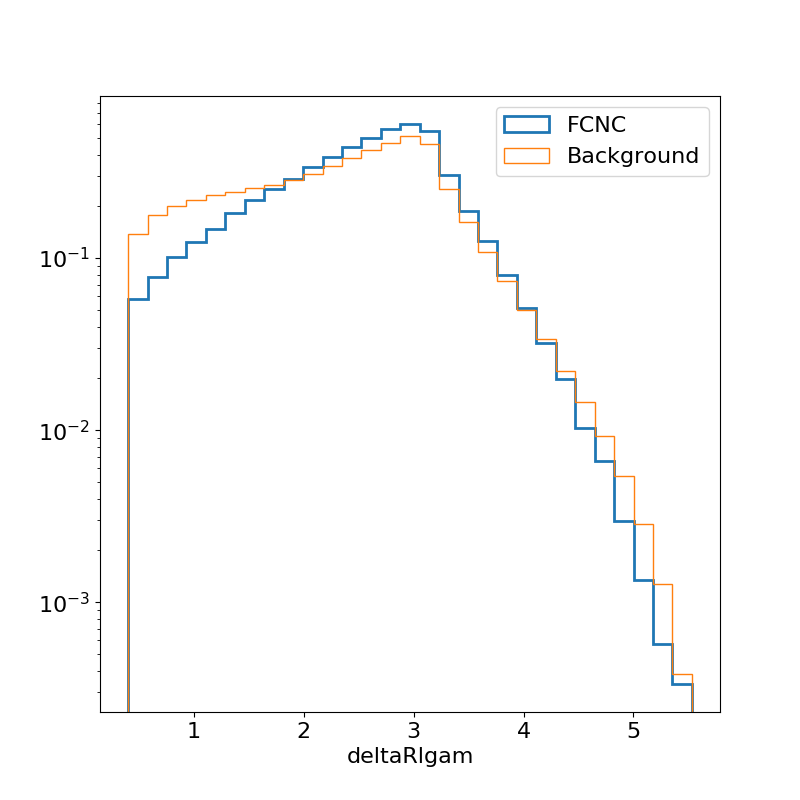
\includegraphics[width=.4\columnwidth]{../ThesisImages/SearchStrategy/varplots/deltaRlgam.png}}\hfil
\subfloat[E (lepton)]{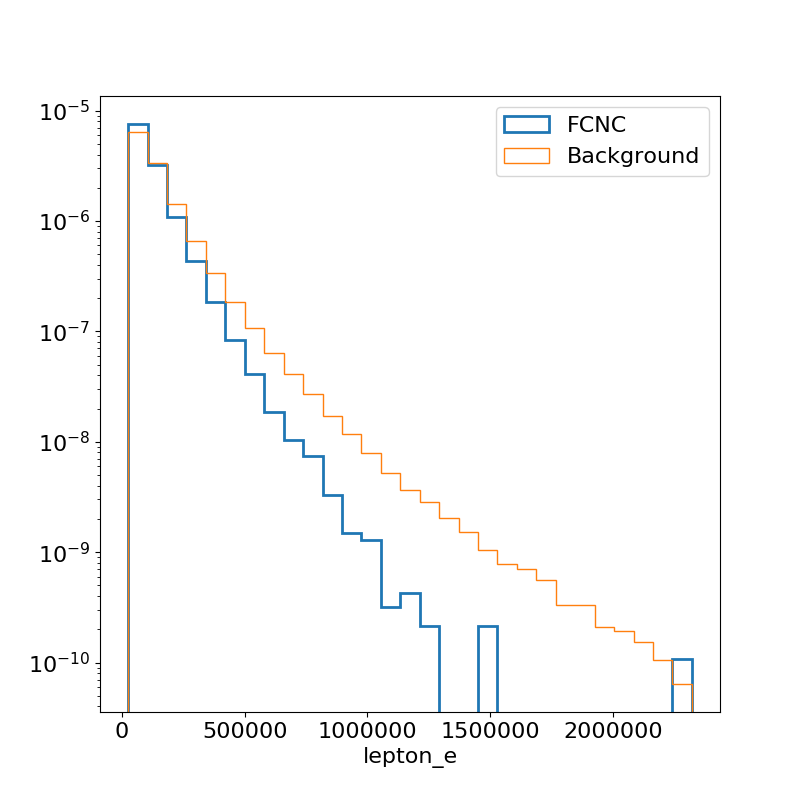
\includegraphics[width=.4\columnwidth]{../ThesisImages/SearchStrategy/varplots/lepton_e.png}}
\vspace{-4.5mm}
\subfloat[$\slashed{E}_T  $]{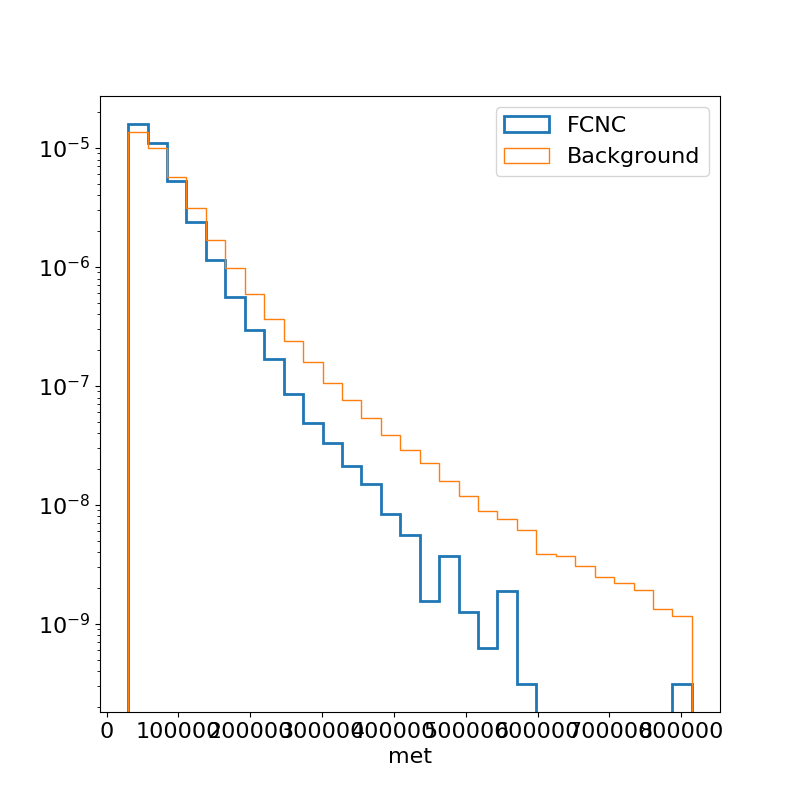
\includegraphics[width=.4\columnwidth]{../ThesisImages/SearchStrategy/varplots/met.png}}\hfil
\subfloat[$p_T (b)$ ]{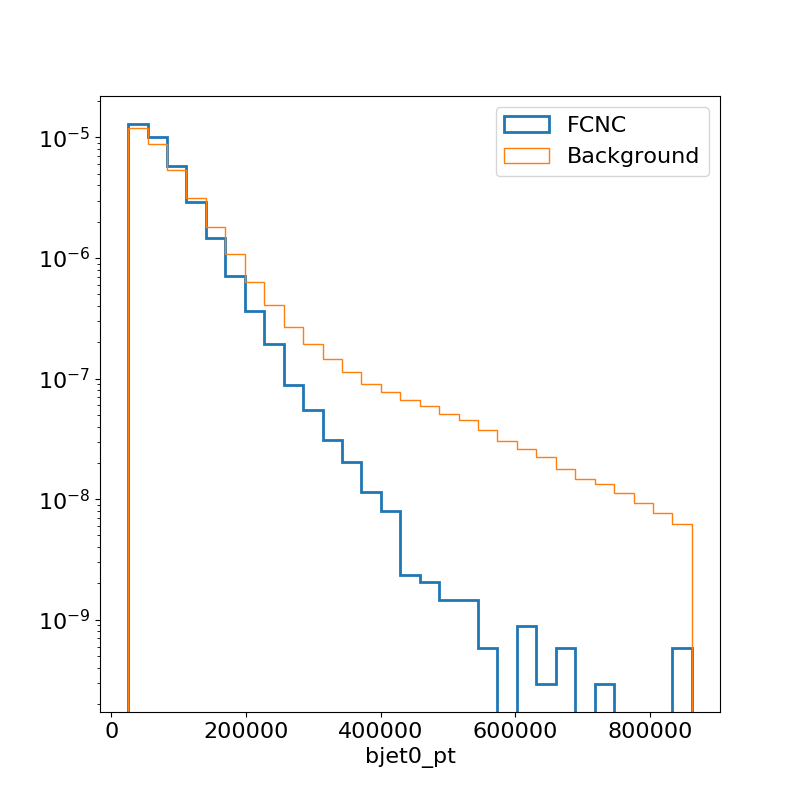
\includegraphics[width=.4\columnwidth]{../ThesisImages/SearchStrategy/varplots/bjet0_pt.png}}   
\caption{Normalized variables showing the shapes of neural network input variables for the $\mu$+jets channel: $\Delta R_{l \gamma}$, E (lepton), $\slashed{E}_T  $, and $p_T (b)$}
\label{fig:VarPlots3}
\end{figure}


\subsection{Architecture}

A variety of architecures of dense neural networks are studied using \textsc{Keras}\cite{Keras} on top of the \textsc{TensorFlow} backend \cite{TensorFlow}.  Each network has a number of input nodes equal to the number of input variables.  Networks with one, two, and three hidden layers are investigated each with 20 nodes.  The output layer contains only a single node.  Every node in one layer is connected to every node in the next layer and the previous layer.  Every connection is assigned a weight that is optimized during the training of the network.  For every node in the network a value is computed using the weights and input values of the previous nodes using an activation function.  Nodes with the highest output of this function are more important to the fit.  The activation function used on the internal nodes in this search is the Rectified Linear Unit activation function.
\[ ReLU(x) = 
\begin{cases}
x, \qquad \text{if } x \geq 0\\
0, \qquad \text{if } x < 0
\end{cases}
\]
The output layer uses the sigmoid function, $\sigma(x)$, as an activation function.  The sigmoid function maps the output smoothly to the range (0,1).
\[ \sigma(x) = \frac{1}{1+e^{-x}}
\]
Every training step the weights of each node are updated following an optimization algorithm, in this case the \textsc{Adam} optimizer\cite{AdamOpt}.  This optimizer follows the steepest gradient to reach the minimum of the parameter of interest called the loss function.  The loss function used for these classification neural networks is the binary cross entropy:
\[\text{Loss} = -\frac{1}{N}\sum_{i=1}^{N}y_{i} \text{log}(p(y_{i}))+(1-y_{i})\text{log}(1-p(y_{i}))\]
where y is a binary indicator (0 or 1) if class label is the correct classification for observation and p is the predicted probability observation is the class label (0 or 1).  The logarithmic nature of this loss function means it applys small values to correctly assigned event but more harshly punishes mismatching of events.  Therefore having a similar number of signal and background events that get weighted similarly can improve the behavior of the network.  In rare decay searches typically the amount of signal events is significantly smaller than the amount of background events in the training sample.  Using the weight functionality in keras the total number of signal events can be scaled to be similar to the number of background events. 

Weighting the signal events this way allows the network to separate the signal and background events in a way that is significantly less harsh than without the weights by taking advantage of the loss function being used.  This improves the estimated significance of the neural network cut after the signal events are rescaled to their proper normalization values.  

\begin{figure}[h!]
	\centering
	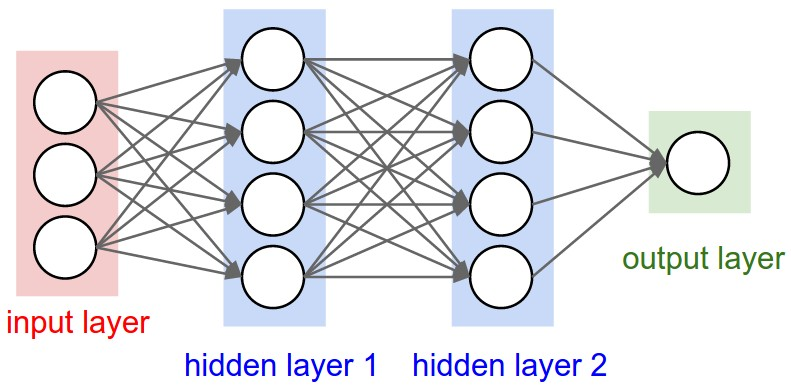
\includegraphics[width=\columnwidth]{../ThesisImages/SearchStrategy/neural_net2.jpeg}
	\caption[Pictoral representation of neural network architecture with 3 input variables, 2 hidden layers with 4 nodes each, and 1 output layer.]{Pictoral representation of neural network architecture with 3 input variables, 2 hidden layers with 4 nodes each, and 1 output layer\cite{NNImage}.}
	\label{fig:NNArch}
\end{figure}

Various hyperparameters are used as inputs into the neural network as well as the optimizer used.  The \textsc{Adam} optimizer has a default learning rate of 0.001 which was not changed throughout these studies.   The learning rate corresponds to the amount that weights are updated during training.  A learning rate that is too large can mean the network never settles into a local minima as it is always missing the minima or at the very least it can take much longer to converge into a minima.  As the neural network training for this search always converged quickly and to a similar value after being tested multiple different times the learning rate was not adapted.  

Another hyperparameter of note is the batch size which defines the number of samples that are propagated through the network at once.  The batch size is of crucial importance in how long the training of the network takes.  A set of 1000 training samples with a batch size of 100 will propagate each set of 100 samples through the neural network every epoch, so 10 separate batches.  A larger batch size means that each epoch of the training takes a shorter amount of time.  However, as the weights are updated after each batch the network can take many more epochs to converge as the weights are being updated less frequently.  A batch size of 100 was used while training the networks presented in this chapter.  Larger batch sizes were tested with the only difference being the time each epoch took and the total time the network took to converge.

Epochs are the total number of times the network has been trained over the entire training set.  All of the networks were allowed up to 200 epochs to converge with a \textsc{keras} patience value set to 50.  The loss function minimization would be done every batch and after each epoch the best possible value of the loss function is found.  If this value is better than any previous epoch the network is allowed to train for 50 more epochs until 50 epochs have passed without finding a new minimum loss function value which then terminates the training.  All models converge early and are terminated typically between epoch 80 and 120 meaning the loss function was minimized between epoch 30 and 70.  

One method employed to avoid overtraining the network dropout regularization was used on each of the hidden layers.  Dropout has the effect of simulating a large number of networks with very different network structures by removing nodes randomly throughout the training. A dropout rate of 20\% was used meaning that for every batch 20\% of the weights of the hidden layer nodes were set to 0.  This forces the network to not become overly dependent on any given node and learning the data `by heart' as opposed to recognizing the trends in the sample. 

\subsubsection{Training and Validation of Neural Networks}

The input variables into the neural network are preprocessed using the \textsc{RobustScalar} method implemented in \textbf{scikit-learn}\cite{ScikitLearn}.  The preprocessing is done so that the input variables exist on a similar scale.  As the network is tasked with learning how to combine these inputs through a series of linear combinations and nonlinear activation function values a disparity in the scales of the input values can lead to awkward loss function topology that will focus on certain parameter gradients instead of treating them all similarly.  Normalizing the values to a standard scale allows the network to learn the optimal parameters for each input node more quickly and efficiently.  This means that less focus can be used on the optimization of the hyperparameters for the network as the scales of the inputs do not need to be learned by the network itself.

Each input variable in the neural network, $x$, is scaled by the following equation:
\[ z = \frac{x - m }{q_3 - q_1} \]
where $m$ is the median of the distribution, $q_1$ and $q_3$ are the first and third quartile.  This changes the distribution of the input variable distributions to be centered around zero.

A second method to avoid overtraining the neural network is to make use of a train-test split to split the signal and background samples into 3 independent randomized sets before training the neural network.  The samples are split into a training set of 64\% of the samples, a test set  containing 20\% of the samples, and the remaing 16\% are a validation set.  The training and test sets are used during the training of the network while the validation set is used to compute performance of the trained neural network.

One measure of the performance of the network is the accuracy. The \textsc{Keras} default accuracy measure is defined:
\[ \text{accuracy} = \frac{N(\text{event}_{NN} \geq 0.5|\text{signal})+ N(\text{event}_{NN} <0.5|\text{background})}{N(\text{signal})+N(\text{background})} \]
where $N(\text{event}_{NN} \geq 0.5|\text{signal})$ ($N(\text{event}_{NN} \geq 0.5|\text{signal})$) is the number of signal (background) events with $P_{\text{signal}}\geq 0.5$ ($P_{\text{signal}}< 0.5$).  Essentially, the accuracy is a measure of the mean of how often correct prediction values occur assuming a cut on the output of $\geq0.5$.

% EJets Train Test Split
% train, test, val
% Sig: (72589, 47) (22685, 47) (18148, 47)
%ttbar (963721, 47) (301163, 47) (240931, 47)
%singleTop (56456, 47) (17643, 47) (14114, 47)
%ttV (190610, 47) (59566, 47) (47653, 47)
%diboson (68024, 47) (21258, 47) (17007, 47)
%WJets (195049, 47) (60953, 47) (48763, 47)
%ZJets (314462, 47) (98270, 47) (78616, 47)
%Mujets train Test Val
%Sig: (75607, 47) (23628, 47) (18902, 47)
%ttbar (912851, 47) (285266, 47) (228213, 47)
%singleTop (53772, 47) (16804, 47) (13444, 47)
%ttV (153174, 47) (47868, 47) (38294, 47)
%diboson (45536, 47) (14231, 47) (11384, 47)
%WJets (189872, 47) (59335, 47) (47468, 47)
%ZJets (104734, 47) (32730, 47) (26184, 47)
% 80% train, 20% test
% 80% newtrain, 20% val

%%%%%%%%%% Show outputs for a network, give examples all my pretty plots

\subsection{Hidden Layer Studies}
\label{sec:HiddenStudies}
The general performance of the neural network was studied with a varying number of hidden layers (1, 2, and 3) in both the $e$+jets and $\mu$+jets channels.   All of the networks are trained on the same set of variables and with the same train-test split input data.  For each of the channels the \textit{Receiver Operating Charactersitic} (ROC) curves are shown in Figure \ref{fig:ROCHidden}.  The ROC curves show the value of $1-\epsilon_{\text{bkg}}$ as a function of the true positive rate, $\epsilon_{\text{signal}}$.  A figure of merit is the Area Under the Curve (AUC) which is a measure of how close the resulting values are to the optimal value of unity. 

\begin{figure}[h!]
\centering
\subfloat[$e$+jets ROC Curves]{\includegraphics[width=.5\columnwidth]{../ThesisImages/SearchStrategy/{HiddenLayerStudiesBR0.002}/btag77/modelouts/ejetsbothroc.png}}\hfil
\subfloat[$\mu$+jets ROC Curves]{\includegraphics[width=.5\columnwidth]{../ThesisImages/SearchStrategy/{HiddenLayerStudiesBR0.002}/btag77/modelouts/mujetsbothroc.png}}
\caption{ROC Curves are shown for both search channels for a varying number of hidden layers. Orange lines correspond to one hidden layer, blue to 2 hidden layers and green to 3 hidden layers.  The blue and green curves have near identical AUC values: 0.950 and 0.951 for the $e$+jets case and $0.962$ for the $\mu$+jets cases.}
\label{fig:ROCHidden}
\end{figure}

The AUC for 2 hidden layers and 3 hidden layers are identical, to rounding errors, for both channels.  As such the network with 2 hidden layers has been chosen as it is computationally simpler.   The normalized neural network output values are shown in Figure \ref{fig:HiddenSigBkg}.  Adding a second hidden layer significantly improves the performance of the network but a third layer does not.  The output shapes change slightly adding the third hidden layer due to the network learning differently about the same data.  However, as the AUC shows, the performance of 2 and 3 hidden layers is identical.   Figures \ref{fig:Acc2Hid} and \ref{fig:Loss2Hid} show the accuracy metric and the loss function as a function of the training epoch for the networks trained with 2 hidden layers.   The accuracy plot behavior is expected as the validation data sets do not have dropout regularization applied to them.  These networks are also trained without further reduction of Z+jets background meaning the $e$+jets sample has a larger background contamination that makes the validation testing more volatile.  This is due to the increased number of similar events in that sample that can be more heavily dependent on specific weights across the network for identification.

\begin{figure}[h!]
\centering
\subfloat[$e$+jets Accuracy Curves]{\includegraphics[width=.5\columnwidth]{../ThesisImages/SearchStrategy/{HiddenLayerStudiesBR0.002}/BestResults/btag77/ejetsboth2hidnpart0accuarcy.png}}\hfil
\subfloat[$\mu$+jets Accuracy Curves]{\includegraphics[width=.5\columnwidth]{../ThesisImages/SearchStrategy/{HiddenLayerStudiesBR0.002}/BestResults/btag77/mujetsboth2hidnpart0accuarcy.png}}
\caption{Accuracy plots for both channels for the 2 hidden layer neural network}
\label{fig:Acc2Hid}
\end{figure}

\begin{figure}[h!]
\centering
\subfloat[$e$+jets Loss Curve]{\includegraphics[width=.5\columnwidth]{../ThesisImages/SearchStrategy/{HiddenLayerStudiesBR0.002}/BestResults/btag77/ejetsboth2hidnpart0loss.png}}\hfil
\subfloat[$\mu$+jets Loss Curve]{\includegraphics[width=.5\columnwidth]{../ThesisImages/SearchStrategy/{HiddenLayerStudiesBR0.002}/BestResults/btag77/mujetsboth2hidnpart0loss.png}}
\caption{Loss plots for both channels for the 2 hidden layer neural network}
\label{fig:Loss2Hid}
\end{figure}

The main metric used in choosing which network has the best physics reach is the significance:
\[ \text{significance} = \frac{N_{s}}{\sqrt{N_s +N_b}}\]
where $N_{s}$ is the number of signal events that pass the cut and $N_b$ is the number of background events that pass the neural network cut.
After the model has been fully trained it is tested on all of the Monte Carlo for signal and background.  The signal samples are normalized to various branching ratios (in the range $10^{-5}\rightarrow 3\times 10^{-3}$) and full LHC Run-2 Luminosity and the significance is calculated as a function of the cut on the output of the neural network $P(\text{signal})$.  The network with the output cut for the smallest branching ratio with a maximum significance of 2 is chosen, a rough estimate of where the expected limit could be set.  The significance as a function of the neural network output cut is shown in Figure \ref{fig:Sig2Hid}.
\begin{figure}[h!]
\centering
\subfloat[$e$+jets:1 Hidden Layer]{\includegraphics[width=.33\columnwidth]{../ThesisImages/SearchStrategy/{HiddenLayerStudiesBR0.002}/btag77/modelouts/ejetsboth1hidnpart0sigbkg.png}}\hfil
\subfloat[$e$+jets:2 Hidden Layers]{\includegraphics[width=.33\columnwidth]{../ThesisImages/SearchStrategy/{HiddenLayerStudiesBR0.002}/btag77/modelouts/ejetsboth2hidnpart0sigbkg.png}}\hfil
\subfloat[$e$+jets:3 Hidden Layers]{\includegraphics[width=.33\columnwidth]{../ThesisImages/SearchStrategy/{HiddenLayerStudiesBR0.002}/btag77/modelouts/ejetsboth3hidnpart0sigbkg.png}}
\vspace{-3.mm}
\subfloat[$\mu$+jets:1 Hidden Layer]{\includegraphics[width=.33\columnwidth]{../ThesisImages/SearchStrategy/{HiddenLayerStudiesBR0.002}/btag77/modelouts/mujetsboth1hidnpart0sigbkg.png}}\hfil
\subfloat[$\mu$+jets:2 Hidden Layers]{\includegraphics[width=.33\columnwidth]{../ThesisImages/SearchStrategy/{HiddenLayerStudiesBR0.002}/btag77/modelouts/mujetsboth2hidnpart0sigbkg.png}}\hfil
\subfloat[$\mu$+jets:3 Hidden Layers]{\includegraphics[width=.33\columnwidth]{../ThesisImages/SearchStrategy/{HiddenLayerStudiesBR0.002}/btag77/modelouts/mujetsboth3hidnpart0sigbkg.png}}
\caption{Normalized neural network output signal and background distribution plots are shown for both search channels for a varying number of hidden layers.}
\label{fig:HiddenSigBkg}
\end{figure}

\begin{figure}[h!]
\centering
\subfloat[$e$+jets]{\includegraphics[width=.5\columnwidth]{../ThesisImages/SearchStrategy/{HiddenLayerStudiesBR0.002}/BestResults/btag77/significanceejetsboth2hidnpart02.png}}\hfil
\subfloat[$\mu$+jets]{\includegraphics[width=.5\columnwidth]{../ThesisImages/SearchStrategy/{HiddenLayerStudiesBR0.002}/BestResults/btag77/significancemujetsboth2hidnpart02.png}}
\caption[Significance plots for both channels for the 2 hidden layer neural network.]{Significance plots for both channels for the 2 hidden layer neural network.  The green points correspond to a branching ratio with a maximum significance of 5, the orange to a maximum significance of 2.  The $e$+jets ($\mu$+jets) branching ratio with max significance of 2 is $1.22 \times10^{-5} (1.18\times10^{-5})$. The blue, red, purple, and brown points correspond to branching ratios of  $1\times10^{-5}$, $5\times10^{-4}$, $1\times10^{-3}$, and $5\times10^{-3}$, respectively.}
\label{fig:Sig2Hid}
\end{figure}


\subsection{B-Tagging Working Point Studies}
\label{sec:btagNN}
The b-tagging working point selection was also done with similar neural network studies.  Three neural networks were trained with the datasets using the jet information and total scaled events for each of the major b-tagging working points: 70\%, 77\%, and 85\%.  Changing the working point changes a number of things about the signal and background data sets such as which jets are b tagged and therefore which jets are combined into the higher level variables (e.g., $m_{q\gamma}$ and $m_{Wb}$).  The total number of events that pass the preselection to the neural network are also changed for all of the datasets since the neural network are only trained on events with 1 b-tagged jet.  Similar sets of plots to Section \ref{sec:HiddenStudies} will be presented in this section.

This selection of neural networks were trained in parallel with one, two, and three hidden layers.  The only results shown are the 2 hidden layer outputs as they preform equally or better to the others as previously discussed.  The accuracy and loss plots for these networks are shown in Figures \ref{fig:BTagEAccLoss} and \ref{fig:BTagMuAccLoss}.  Following that the neural network output and significance plots are shown in Figures \ref{fig:BTagEOutSig} and \ref{fig:BTagMuOutSig}.  

\begin{figure}[h!]
\centering
\subfloat[70\% WP Loss]{\includegraphics[width=.33\columnwidth]{../ThesisImages/SearchStrategy/{HiddenLayerStudiesBR0.002}/BestResults/btag70/ejetsboth2hidnpart0loss.png}}\hfil
\subfloat[77\% WP Loss]{\includegraphics[width=.33\columnwidth]{../ThesisImages/SearchStrategy/{HiddenLayerStudiesBR0.002}/BestResults/btag77/ejetsboth2hidnpart0loss.png}}\hfil
\subfloat[85\% WP Loss]{\includegraphics[width=.33\columnwidth]{../ThesisImages/SearchStrategy/{HiddenLayerStudiesBR0.002}/BestResults/btag85/ejetsboth2hidnpart0loss.png}}
\vspace{-3.mm}
\subfloat[70\% WP Accuracy]{\includegraphics[width=.33\columnwidth]{../ThesisImages/SearchStrategy/{HiddenLayerStudiesBR0.002}/BestResults/btag70/ejetsboth2hidnpart0accuarcy.png}}\hfil
\subfloat[77\% WP Accuracy]{\includegraphics[width=.33\columnwidth]{../ThesisImages/SearchStrategy/{HiddenLayerStudiesBR0.002}/BestResults/btag77/ejetsboth2hidnpart0accuarcy.png}}\hfil
\subfloat[85\% WP Accuracy]{\includegraphics[width=.33\columnwidth]{../ThesisImages/SearchStrategy/{HiddenLayerStudiesBR0.002}/BestResults/btag85/ejetsboth2hidnpart0accuarcy.png}}
\caption{Accuaracy and loss plots for the $e$+jets channel at 70\%, 77\%, and 85\% b-tagging working points.}
\label{fig:BTagEAccLoss}
\end{figure}

\begin{figure}[h!]
\centering
\subfloat[70\% WP Loss]{\includegraphics[width=.33\columnwidth]{../ThesisImages/SearchStrategy/{HiddenLayerStudiesBR0.002}/BestResults/btag70/mujetsboth2hidnpart0loss.png}}\hfil
\subfloat[77\% WP Loss]{\includegraphics[width=.33\columnwidth]{../ThesisImages/SearchStrategy/{HiddenLayerStudiesBR0.002}/BestResults/btag77/mujetsboth2hidnpart0loss.png}}\hfil
\subfloat[85\% WP Loss]{\includegraphics[width=.33\columnwidth]{../ThesisImages/SearchStrategy/{HiddenLayerStudiesBR0.002}/BestResults/btag85/mujetsboth2hidnpart0loss.png}}
\vspace{-3.mm}
\subfloat[70\% WP Accuracy]{\includegraphics[width=.33\columnwidth]{../ThesisImages/SearchStrategy/{HiddenLayerStudiesBR0.002}/BestResults/btag70/mujetsboth2hidnpart0accuarcy.png}}\hfil
\subfloat[77\% WP Accuracy]{\includegraphics[width=.33\columnwidth]{../ThesisImages/SearchStrategy/{HiddenLayerStudiesBR0.002}/BestResults/btag77/mujetsboth2hidnpart0accuarcy.png}}\hfil
\subfloat[85\% WP Accuracy]{\includegraphics[width=.33\columnwidth]{../ThesisImages/SearchStrategy/{HiddenLayerStudiesBR0.002}/BestResults/btag85/mujetsboth2hidnpart0accuarcy.png}}
\caption{Accuaracy and loss plots for the $\mu$+jets channel at 70\%, 77\%, and 85\% b-tagging working points.}
\label{fig:BTagMuAccLoss}
\end{figure}

\begin{figure}[h!]
\centering
\subfloat[70\% WP NN output]{\includegraphics[width=.33\columnwidth]{../ThesisImages/SearchStrategy/{HiddenLayerStudiesBR0.002}/BestResults/btag70/ejetsboth2hidnpart0sigbkg.png}}\hfil
\subfloat[77\% WP NN output]{\includegraphics[width=.33\columnwidth]{../ThesisImages/SearchStrategy/{HiddenLayerStudiesBR0.002}/BestResults/btag77/ejetsboth2hidnpart0sigbkg.png}}\hfil
\subfloat[85\% WP NN output]{\includegraphics[width=.33\columnwidth]{../ThesisImages/SearchStrategy/{HiddenLayerStudiesBR0.002}/BestResults/btag85/ejetsboth2hidnpart0sigbkg.png}}
\vspace{-3.mm}
\subfloat[70\% WP Significance]{\includegraphics[width=.33\columnwidth]{../ThesisImages/SearchStrategy/{HiddenLayerStudiesBR0.002}/BestResults/btag70/significanceejetsboth2hidnpart02.png}}\hfil
\subfloat[77\% WP Significance]{\includegraphics[width=.33\columnwidth]{../ThesisImages/SearchStrategy/{HiddenLayerStudiesBR0.002}/BestResults/btag77/significanceejetsboth2hidnpart02.png}}\hfil
\subfloat[85\% WP Significance]{\includegraphics[width=.33\columnwidth]{../ThesisImages/SearchStrategy/{HiddenLayerStudiesBR0.002}/BestResults/btag85/significanceejetsboth2hidnpart02.png}}
\caption{Neural network output and significance plots for the $e$+jets channel at 70\%, 77\%, and 85\% b-tagging working points.}
\label{fig:BTagEOutSig}
\end{figure}

\begin{figure}[h!]
\centering
\subfloat[70\% WP NN output]{\includegraphics[width=.33\columnwidth]{../ThesisImages/SearchStrategy/{HiddenLayerStudiesBR0.002}/BestResults/btag70/mujetsboth2hidnpart0sigbkg.png}}\hfil
\subfloat[77\% WP NN output]{\includegraphics[width=.33\columnwidth]{../ThesisImages/SearchStrategy/{HiddenLayerStudiesBR0.002}/BestResults/btag77/mujetsboth2hidnpart0sigbkg.png}}\hfil
\subfloat[85\% WP NN output]{\includegraphics[width=.33\columnwidth]{../ThesisImages/SearchStrategy/{HiddenLayerStudiesBR0.002}/BestResults/btag85/mujetsboth2hidnpart0sigbkg.png}}
\vspace{-3.mm}
\subfloat[70\% WP Significance]{\includegraphics[width=.33\columnwidth]{../ThesisImages/SearchStrategy/{HiddenLayerStudiesBR0.002}/BestResults/btag70/significancemujetsboth2hidnpart02.png}}\hfil
\subfloat[77\% WP Significance]{\includegraphics[width=.33\columnwidth]{../ThesisImages/SearchStrategy/{HiddenLayerStudiesBR0.002}/BestResults/btag77/significancemujetsboth2hidnpart02.png}}\hfil
\subfloat[85\% WP Significance]{\includegraphics[width=.33\columnwidth]{../ThesisImages/SearchStrategy/{HiddenLayerStudiesBR0.002}/BestResults/btag85/significancemujetsboth2hidnpart02.png}}
\caption{Neural network output and significance plots for the $\mu$+jets channel at 70\%, 77\%, and 85\% b-tagging working points.}
\label{fig:BTagMuOutSig}
\end{figure}

The result of these studies is the choice of using the 77\% working point for b-tagged jets.  The branching ratio with significance of 2 is found for each network and reported in Table \ref{tab:BRsAfterNN}.

\begin{table}[]
\begin{center}
{\renewcommand{\arraystretch}{1.2}
\begin{tabular}{ccc}
\hline
B-Tag Working Point  &  $e$+jets Branching Ratio   & $\mu$+jets Branching Ratio  \\  \hline 
70\%            &  $1.25\times10^{-5}$  &  $1.31\times10^{-5}$\\
77\%           &   $1.23\times10^{-5}$ &   $1.18\times10^{-5}$	\\  
85\%            &  $1.27\times10^{-5}$ &   $1.19\times10^{-5}$	\\ \hline
\end{tabular}
\caption{Branching ratio values with a significance of 2 after neural network optimization}
\label{tab:BRsAfterNN}
}
\end{center}
\end{table}


%\subsection{Comparison of FCNC in Decay and Production via the Neural Network}

%%%%%%%%%%%%%%%%%%%%%%%%%%%%%%%%%%%%%%%%%%%%%%
%%%%%%%%%  									        	 %%%%%%%%
%%%%%%%%%                     End of Neural Net Section                                             %%%%%%%%
%%%%%%%%%										 %%%%%%%%
%%%%%%%%%%%%%%%%%%%%%%%%%%%%%%%%%%%%%%%%%%%%%%


\section{Initial Event Selection}

Initial event selection is done to ensure that events that are accepted into the analysis are not contaminated by extremely noisey detector environments and happened during times when the ATLAS detector was accepting events properly.  All of the events  have the same initial set of criteria for determining whether or not the event is looked at any further for this analysis, applying to both MC and Data.  These initial checks are as follows:

\begin{itemize}
\item Only events occuring during runs good for physics
\item Good Calorimeter status: Ensures that the LAr and Tile calorimeters are not experiencing a noise burst at the time of the event
\item Requires a primay vertex to be reconstructed for the event which ensures timing of further reconstructed objects are placed with the correct vertex
\item Global Trigger Decision: Selects events based on wheter they passed one of the triggers including the trigger thresholds, further discussion in Section \ref{sec:GTRIGDEC}
\item Trigger Match: Select events where an electron or muon matches the trigger
\item Overlap Removal as discussed in Section \ref{sec:OverlapRemoval}
\item Ignore events that have a bad muon, occurs mostly in the transition region and the cathode strip chamber regions.
\item Jet Cleaning: Removes events with jets formed from calorimeter information from sources that have nothing to do with the energy flow from the initial hard scatter interaction
\end{itemize}

These basic event selection values are applied to every event, in both MC and Data.  On top of these various kinematic cuts are added to form the additional analysis level objects and regions used in the analysis.  These additional kinematic cuts are examined more closely in Section \ref{sec:preselcuts} and in the discussion of region creation throughout the rest of the analysis e.g., Section \ref{sec:BkgEvalCRVR}.


\subsection{Triggers}
\label{sec:GTRIGDEC}
Different HLT triggers are used for data taking periods for each year of Run 2.  This analysis takes advantage of single lepton triggers for electrons and muons to dramatically reduce backgrounds due to QCD events without leptons.  

\begin{table}[]
\small
\begin{center}
{\renewcommand{\arraystretch}{1.2}
\begin{tabular}{c|c|c|c|c}
\hline
Year  &  $p_T$ threshold [GeV]   & Identification Menu & Isolation menu & L1 Seed  \\  \hline 
2015   &    $\geq 24  $ &  Medium  &  None	& L1EM20VH	\\
           &   $\geq 60   $ &   Medium  &  None	&  -	\\  
            &  $\geq 120 $ &   Loose  &    None		& -	\\ \hline 
  &   $\geq 26   $ &  Tight  &   Gradient (Loose) 	&  -	\\
2016-2018  &   $\geq 60   $ &   Medium  &  None	&  -	\\  
 &  $\geq 140 $ &   Loose  &  None	&  -	 \\ \hline     
\end{tabular}
\caption{The electron trigger requirements in the event selections}
\label{tab:ElectronTrigs}
}
\end{center}
\end{table}

\begin{table}[]
\small
\begin{center}
{\renewcommand{\arraystretch}{1.2}
\begin{tabular}{c|c|c|c|c}
\hline
Year  &  $p_T$ threshold [GeV]   & Identification Menu & Isolation menu & L1 Seed  \\  \hline 
2015   &    $\geq 20  $ & None  &  Gradient (Loose)	& L1MU15 \\
           &   $\geq 50   $ &   None  &  None	&  -	\\   \hline 
2016-2018  &   $\geq 26   $ &  None  &   Gradient (Medium) 	&  -	\\
  &   $\geq 50   $ &   None  &  None	&  -	\\ \hline   
\end{tabular}
\caption{The muon trigger requirements in the event selections}
\label{tab:MuonTrigs}
}
\end{center}
\end{table}



\section{Data and MC Pre-Selection Cuts}
\label{sec:preselcuts}
The Signal Region pre-selection is defined to select events that have an opportunity to enter the final search selection.  This pre-selection selects events with exactly one massive lepton, at least two jets (at least one of which is b-tagged at the 77\% working point), transverse momentum and exactly one photon such that it resembles the expected final-state toplogy for the signal.  All of the events have the same initial set of criteria for determining whether or not the event is looked at any further for this analysis, applying to both MC and Data.  These initial checks are as follows:
%% Preselection Itemization
\begin{itemize}
\item
\end{itemize}
%%SR Pre Selection Plots
Pre Selection Plots

\section{Background Evaluation: Control and Validation Regions}
\label{sec:BkgEvalCRVR}
\subsection{Backgrounds Without Photons}
\label{sec:BKGnoPho}

For scale factors

\subsection{Background With Photons}
\label{sec:BKGPho}

\section{Fake Rates}
\subsection{Jet $\rightarrow$ Lepton Fakes}
\label{sec:FakeLep}

\subsection{Electron $\rightarrow$ Photon Fakes}
\label{sec:FakePho}

\subsection{Jet $\rightarrow$ Photon Fakes}
\label{sec:FakePho2}

\section{Signal Region}















%
%### <<<<< settings for mc16a >>>>>
%GRLDir  GoodRunsLists
%GRLFile data15_13TeV/20170619/physics_25ns_21.0.19.xml data16_13TeV/20180129/physics_25ns_21.0.19.xml
%PRWConfigFiles_FS dev/AnalysisTop/PileupReweighting/user.iconnell.Top.PRW.MC16a.FS.v2/prw.merged.root
%PRWConfigFiles_AF dev/AnalysisTop/PileupReweighting/user.iconnell.Top.PRW.MC16a.AF.v2/prw.merged.root
%PRWLumiCalcFiles GoodRunsLists/data15_13TeV/20170619/PHYS_StandardGRL_All_Good_25ns_276262-284484_OflLumi-13TeV-008.root GoodRunsLists/data16_13TeV/20180129/PHYS_StandardGRL_All_Good_25ns_297730-311481_OflLumi-13TeV-009.root
%### <<<<< settings for mc16a >>>>>
%
%# ### <<<<< settings for mc16d >>>>>
%# GRLDir  GoodRunsLists
%# GRLFile data17_13TeV/20180619/physics_25ns_Triggerno17e33prim.xml
%# PRWConfigFiles_FS dev/AnalysisTop/PileupReweighting/user.iconnell.Top.PRW.MC16d.FS.v2/prw.merged.root
%# PRWConfigFiles_AF dev/AnalysisTop/PileupReweighting/user.iconnell.Top.PRW.MC16d.AF.v2/prw.merged.root
%# PRWLumiCalcFiles GoodRunsLists/data17_13TeV/20180619/physics_25ns_Triggerno17e33prim.lumicalc.OflLumi-13TeV-010.root
%# ### <<<<< settings for mc16d >>>>>
%
%# ### <<<<< settings for mc16e >>>>>
%# GRLDir  GoodRunsLists
%# GRLFile data18_13TeV/20190318/physics_25ns_Triggerno17e33prim.xml
%# PRWConfigFiles_FS dev/AnalysisTop/PileupReweighting/user.iconnell.Top.PRW.MC16e.FS.v2/prw.merged.root
%# PRWConfigFiles_AF dev/AnalysisTop/PileupReweighting/user.iconnell.Top.PRW.MC16e.AF.v2/prw.merged.root
%# PRWLumiCalcFiles GoodRunsLists/data18_13TeV/20190318/ilumicalc_histograms_None_348885-364292_OflLumi-13TeV-010.root
%
%

%

%










%%%%%%%%